\section{Trägheitsmoment und Rotationsenergie}
Wir wollen jetzt allgemein die Rotationsenergie von Körpern beschreiben, unter der Einschränkung, dass ihre Bewegung die ganze Zeit in der Ebene stattfindet.
\begin{figure}
  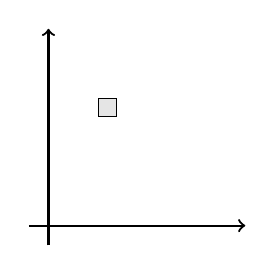
\begin{tikzpicture}
    \draw[->,thick] (-.25,0) -- (2.5,0);
    \draw[->,thick] (0,-.25) -- (0,2.5);
    \node[rectangle, draw, fill=gray!20] at (.75,1.5) {};
  \end{tikzpicture}
  \caption{}
  \label{}
\end{figure}
